\pdfminorversion=6
\documentclass{report}
\usepackage{amsmath, amssymb, amsthm}
\usepackage{titlesec}
\titleformat{\chapter}{\bfseries\LARGE}{\thechapter.~}{0em}{}
\usepackage{comment}

\usepackage[english]{babel}
\usepackage{blindtext}

\usepackage{graphicx}
\graphicspath{ {./Figures/} }

\begin{document}

\title{Regulator based meshed LVDC distribution network}
\author{Tomi Lotila}
\maketitle

\tableofcontents


\listoffigures

% This chapter should answer the following questions.
 % What is in this paper?
 % Which questions does this paper answers?
\chapter{Introduction}
The traditional LVAC distribution network is based on a unidirectional radial design, which limits the distributed energy resource (DER) integration. In contrast, a meshed LVDC distribution network is a multi-source, multi-load topology that allows bidirectional power flow and easy DER integration.

One of the key challenges in the implementation of meshed network is maintaining power flow control. This can be achieved by using a direct current (DC) regulators, which are a devices that can control the current and power flow.

The main objective of this paper is to design, simulate, and evaluate a regulator-based meshed DC network, and to investigate its performance under different operating conditions. The current regulator desgins discussed in this paper are suitable for low voltage only.










% Additional sources:
 % https://energycentral.com/c/iu/mesh-networks-short-introduction



% This chapter should answer the following questions.
\chapter{Direct current transmission system}
% What is direct current transmission system, and LV-/HVDC
Direct Current (DC) power systems are electrical power systems that utilize a constant voltage level, and are characterized by a steady and unidirectional flow of electric current. 

DC power systems can be classified into two types: low voltage DC power systems and high voltage DC power systems. Low voltage DC power systems have a voltage level of less than 1,500 V and are used in small electronic devices, and electric vehicles \cite{IEC60038}. High voltage DC power systems have a voltage level of more than 1,500 V and are mainly used in industrial applications, such as long-distance power transmission.


\begin{comment}

potential sources
[1] J. Grainger and W. Stevenson, Power System Analysis, McGraw-Hill, 1994.
[2] T.A. Short, Power System Stability and Control, IEEE Press, 1993.
[3] J.K. Saini and P. Kundur, Power System Stability and Control, CRC Press, 2007.
[4] R. Lasseter and G. Andhankar, "Microgrids and Active Distribution Networks," IEEE Power and Energy Magazine, vol. 11, no. 3, pp. 40-50, 2013.
\end{comment}
% what limits power transmission capacity
\paragraph{} Power transmission in DC transmission lines are limited by two factors, power line thermal limitation and voltage stability.

Power line thermal limitation refers to the maximum amount of power that can be transmitted over a power line without causing damage to the line or creating unsafe conditions. The thermal limit of a power line is determined by the maximum temperature that the line and its insulation can withstand without suffering damage.

The thermal limit of a power line is affected by several factors, including the size and material of the conductor, the type and thickness of the insulation, the ambient temperature, the altitude. The thermal limit of a power line is usually determined by the manufacturer and is specified in the technical data sheet for the line.

Exceeding the thermal limit of a power line can cause damage to the line and create unsafe conditions. Therefore, it is important to ensure that the thermal limit of a power line is not exceeded during normal and abnormal operating conditions. This can be done by monitoring the temperature of the line and the ambient conditions, and by controlling the amount of power transmitted over the line.

Voltage stability in DC power transmission systems refers to the ability of the system to maintain a stable voltage level at all buses under all times.  Variations in the load demand or in the power generation should not have significant effect on voltage level. Power systems have voltage level margin, for example in Finland it is +-5\% of the nominal voltage.

Voltage stability is crucial for the operation of the DC power transmission systems because it affects the ability of the system to transfer power and maintain power quality.







\begin{comment}

potential sources
[1] J. Grainger and W. Stevenson, Power System Analysis, McGraw-Hill, 1994.
[2] T.A. Short, Power System Stability and Control, IEEE Press, 1993.
[3] J.K. Saini and P. Kundur, Power System Stability and Control, CRC Press, 2007.
[4] R. Lasseter and G. Andhankar, "Microgrids and Active Distribution Networks," IEEE Power and Energy Magazine, vol. 11, no. 3, pp. 40-50, 2013.
\end{comment}


% This chapter should answer the following questions.
 % What is a meshed power grid?
 % Why is meshed grid needed?
 % Is meshed gird already in use?
 % How do meshed- and branched girds differ?
 % How do DC- and AC grids differ?
\chapter{Power distribution network types}
% what type of power distribution networks exists
\input{Chapters/Power distribution network types/what are distribution networks.tex}
\section{Radial distribution network} Radial distribution networks are the most common type of distribution networks and are characterized by a tree-like structure that branches out from a central source to various customers. Power flows in a single direction from the source to the loads. \cite{PowerSystemAnalysis:1994}

\begin{figure}[h]
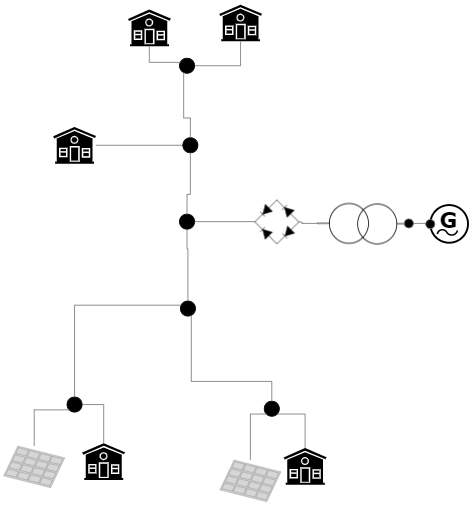
\includegraphics{Radial distribution network.png}
\label{fig:Radial distribution network}
\caption{Radial distribution network}
\end{figure}



\begin{comment}

potential sources
[2] T.A. Short, Power System Stability and Control, IEEE Press, 1993.
[3] J.K. Saini and P. Kundur, Power System Stability and Control, CRC Press, 2007.
[4] R. Lasseter and G. Andhankar, "Microgrids and Active Distribution Networks," IEEE Power and Energy Magazine, vol. 11, no. 3, pp. 40-50, 2013.
\end{comment}
\section{Loop distribution network} Loop distribution network is characterized by a closed loop of transmission line. This allows for two paths for power to flow, increasing the reliability of the system.


\begin{comment}

potential sources

\end{comment}
\section{Meshed distribution network} Meshed distribution network is characterized by a web-like structure of interconnections between transmission lines. This allows for multiple paths for power to flow, increasing the reliability of the system.






\begin{comment}

potential sources

\end{comment}



% This chapter should answer the following questions.
\chapter{Direct current regulators}
Direct current regulator is an electronic circuit that is designed to control  current, even in the presence of changes in input voltage or load resistance. This is achieved by sensing the current flowing through and adjusting the current supplied to the load.

There are several different types of DC regulators, each with their own unique characteristics and applications. They can be separated into linear DC regulators and switch-mode DC regulators, based on how current is controlled.


\begin{comment}
potentiaal sources

https://www.monolithicpower.com/en/voltage-regulator-types
https://www.rohm.com/electronics-basics/dc-dc-converters/linear-vs-switching-regulators
https://en.wikipedia.org/wiki/Pulse-width_modulation#Power_delivery
https://en.wikipedia.org/wiki/Chopper_(electronics)

"Power Electronics: Converters, Applications, and Design" by Ned Mohan, Tore M. Undeland, William P. Robbins.
"Power Electronics Handbook" Edited by Muhammad H. Rashid
"Control of Electric Motors" by William W. Stacey.

\end{comment}
\section{Linear regulators} Linear DC regulators are the most basic type of DC regulator and work by using a voltage reference and an error amplifier to control the output voltage. The output voltage is proportional to the input voltage, and the error amplifier compares the output voltage to the voltage reference to control the input current. Linear regulators are simple, but they are less efficient than other types of DC regulators and can generate significant heat.

Figure \ref{fig:linear_DC_regulator} has a implementation of linear DC regulator. 


\begin{figure}[]
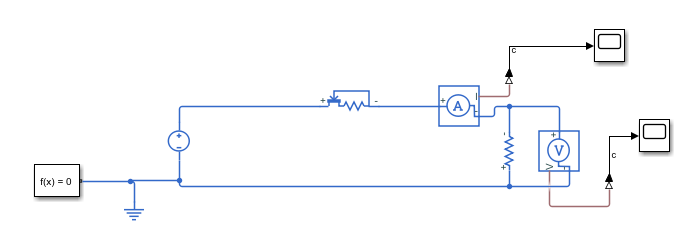
\includegraphics[width=\textwidth]{linear_DC_regulator.png}
\label{fig:linear_DC_regulator}
\caption{Matlab/simulink model of linear DC regulator}
\end{figure}



\begin{comment}

potential sources
https://en.wikipedia.org/wiki/Linear_regulator

\end{comment}
\section{Switch-mode regulators} Switch-mode regulators, on the other hand, use switching technology to control the output voltage. They work by rapidly switching the input voltage on and off, and using a feedback loop to control the switching frequency and duty cycle. Switch-mode regulators are more efficient than linear regulators and can handle larger input-to-output voltage differences, but they are more complex and can generate electromagnetic interference (EMI).

Overall, switch-mode regulators are a useful and versatile technology that offers many benefits for a wide range of electronic applications. They are used in a variety of applications, including power supplies for electronic devices, battery chargers, and voltage converters for automotive and industrial use. Due to their high efficiency and compact size, switch-mode regulators are becoming increasingly popular in portable devices and in applications where space is at a premium.

There are two different switch-mode regulators that could work in meshed network, which are step-down converter and chopper converter.



\begin{comment}

potentiaal sources
"Power Electronics: Converters, Applications, and Design" by Ned Mohan, Tore M. Undeland, William P. Robbins.
"Pulse Width Modulation for Power Converters: Principles and Practice" by Paul C. C. Hwang
"Switching Power Converters: Design and Analysis" by Khalid Sheikh.

\end{comment}
\subsection{Step-down converter} A step-down converter, also known as a buck converter, is a type of switch-mode power converter that is designed to convert a higher input voltage to a lower output voltage. This is achieved by rapidly switching a device, such as a transistor, on and off to regulate the output voltage.

The basic circuit of a step-down converter includes an inductor, a switch, a diode and a capacitor. The inductor stores energy during the on-time of the switch and releases energy to the output during the off-time of the switch. The diode is used to prevent the inductor from discharging energy back to the input. The capacitor is used to filter the output voltage.

Step-down converters have several advantages over traditional linear regulators, including high efficiency, small size and wide input voltage range, which makes them widely used in various electronic devices such as personal computers, mobile phones, tablets, and other portable devices.

However, step-down converters also have some disadvantages, such as the potential for EMI and the need for additional components, such as inductors and capacitors, to filter the output voltage.





\begin{comment}

additional sources
https://en.wikipedia.org/wiki/Buck_converter
"Switching Power Supply Design" by Abraham I. Pressman
"Design of Switching Power Supplies, UPS and Voltage Stabilizers" by Slawomir Tumanski
"Power Electronics: Converters, Applications, and Design" by Ned Mohan, Tore M. Undeland, William P. Robbins.

\end{comment}
\subsection{Chopper converter} A chopper converter is a type of electronic circuit that is used to convert fixed DC voltage to variable DC voltage, usually by chopping a DC input voltage into a train of pulses. The process of chopping is achieved by rapidly switching a device, such as a transistor, on and off to control the output voltage. Essentialy a chopper is a pulse width modulated (PWM) switch.

Chopper converters are used in applications that non-constant power output doesnot  matter, like battery chargers and brushed DC motor speed controllers. For the example of battery charger, charging the battery in pulses or in constant power doesnot make a difference. The reason why chopper converter is used in battery charges is to prevent over heating and over changing of the battery. Similarly, in meshed DC grid, chopper converter could be used to prevent the power line conductors from over heating. DC power quality for customer might be decreased in this scenario.

\begin{comment}

additional sources
https://en.wikipedia.org/wiki/Chopper_(electronics)
"Power Electronics: Converters, Applications, and Design" by Ned Mohan, Tore M. Undeland, William P. Robbins.
"Pulse Width Modulation for Power Converters: Principles and Practice" by Paul C. C. Hwang
"Switching Power Converters: Design and Analysis" by Khalid Sheikh.

\end{comment}

 % This chapter should answer the following questions.
%\chapter{Overview of Power Semiconductor Switches}
%\section{Uncontrolled}
\subsection{diode}
\section{Semi-controlled}
\subsection{thyristor}
\subsection{SCR}
\section{Fully Controlled }
\subsection{BJT}
\subsection{MOSFET}
\subsection{GTO}
\subsection{IQBT}
\section{Comparison}





% Additional sources:
 % 







% This chapter should answer the following questions.
\chapter{Power quality}
\section{power storage}
\subsection{capacitor}
\subsection{super capacitor}
\subsection{lto}
\section{energy storage}
\subsection{lfp}
\subsection{potential energy}
\subsection{kinetic energy}








% Additional sources:
 % 


% This chapter should answer the following questions.
\chapter{Black start of a meshed grid}
\cite{blackStartPracEngineering}
\section{grid forming}





% additional sources
% Overview of black start: https://practical.engineering/blog/2022/12/5/what-is-a-black-start-of-the-power-grid

% This chapter should answer the following questions.
% only full rated converter wind turbine scheme, no fixed speed or double fed induction generator
\chapter{Connecting distributed generation to DC grid}

% This chapter should answer the following questions.
%\chapter{Power flow between AC and DC grids}
%% full bridge rectifier
\section{AC to DC}
% inverter
\section{DC to AC}









% Additional sources:
 % 




\bibliographystyle{plain} 
\bibliography{Chapters/refs.bib} 

\end{document}
